\documentclass[
  bibliography=totoc,     % Literatur im Inhaltsverzeichnis
  captions=tableheading,  % Tabellenüberschriften
  titlepage=firstiscover, % Titelseite ist Deckblatt (Finnd ich nicht so gut)
]{scrartcl}

% Paket float verbessern
\usepackage{scrhack}

% Warnung, falls nochmal kompiliert werden muss
\usepackage[aux]{rerunfilecheck}

% unverzichtbare Mathe-Befehle
\usepackage{amsmath}
% viele Mathe-Symbole
\usepackage{amssymb}
% Erweiterungen für amsmath
\usepackage{mathtools}

%\usepackage{physics}

% Fonteinstellungen
\usepackage{fontspec}
% Latin Modern Fonts werden automatisch geladen
% Alternativ zum Beispiel:
%\setromanfont{Libertinus Serif}
%\setsansfont{Libertinus Sans}
%\setmonofont{Libertinus Mono}

% Wenn man andere Schriftarten gesetzt hat,
% sollte man das Seiten-Layout neu berechnen lassen
\recalctypearea{}

% deutsche Spracheinstellungen
\usepackage[ngerman]{babel}


\usepackage[
  math-style=ISO,    % ┐
  bold-style=ISO,    % │
  sans-style=italic, % │ ISO-Standard folgen
  nabla=upright,     % │
  partial=upright,   % ┘
  warnings-off={           % ┐
    mathtools-colon,       % │ unnötige Warnungen ausschalten
    mathtools-overbracket, % │
  },                       % ┘
]{unicode-math}

% traditionelle Fonts für Mathematik
\setmathfont{Latin Modern Math}
% Alternativ zum Beispiel:
%\setmathfont{Libertinus Math}

\setmathfont{XITS Math}[range={scr, bfscr}]
\setmathfont{XITS Math}[range={cal, bfcal}, StylisticSet=1]

% Zahlen und Einheiten
\usepackage[
  locale=DE,                   % deutsche Einstellungen
  separate-uncertainty=true,   % immer Unsicherheit mit \pm
  per-mode=symbol-or-fraction, % / in inline math, fraction in display math
]{siunitx}

% chemische Formeln
\usepackage[
  version=4,
  math-greek=default, % ┐ mit unicode-math zusammenarbeiten
  text-greek=default, % ┘
]{mhchem}

% richtige Anführungszeichen
\usepackage[autostyle]{csquotes}

% schöne Brüche im Text
\usepackage{xfrac}

% Standardplatzierung für Floats einstellen
\usepackage{float}
\floatplacement{figure}{htbp}
\floatplacement{table}{htbp}

% Floats innerhalb einer Section halten
\usepackage[
  section, % Floats innerhalb der Section halten
  below,   % unterhalb der Section aber auf der selben Seite ist ok
]{placeins}

% Seite drehen für breite Tabellen: landscape Umgebung
\usepackage{pdflscape}

% Captions schöner machen.
\usepackage[
  labelfont=bf,        % Tabelle x: Abbildung y: ist jetzt fett
  font=small,          % Schrift etwas kleiner als Dokument
  width=0.9\textwidth, % maximale Breite einer Caption schmaler
]{caption}
% subfigure, subtable, subref
\usepackage{subcaption}

% Grafiken können eingebunden werden
\usepackage{graphicx}
\usepackage{wrapfig}

% schöne Tabellen
\usepackage{booktabs}

% Verbesserungen am Schriftbild
\usepackage{microtype}

% Literaturverzeichnis
\usepackage[
  backend=biber,
  sorting=none
]{biblatex}
% Quellendatenbank
\addbibresource{lit.bib}
\addbibresource{programme.bib}

% Hyperlinks im Dokument
\usepackage[
  german,
  unicode,        % Unicode in PDF-Attributen erlauben
  pdfusetitle,    % Titel, Autoren und Datum als PDF-Attribute
  pdfcreator={},  % ┐ PDF-Attribute säubern
  pdfproducer={}, % ┘
]{hyperref}
% erweiterte Bookmarks im PDF
\usepackage{bookmark}

% Trennung von Wörtern mit Strichen
\usepackage[shortcuts]{extdash}

%\setcounter{tocdepth}{3} % + subsubsections



\author{%
  Clara Sondermann \\%
  \href{mailto:clara.sondermann@tu-dortmund.de}{clara.sondermann@tu-dortmund.de}%
  \and%
  Enno Wellmann \\%
  \href{mailto:enno.wellmann@tu-dortmund.de}{enno.wellmann@tu-dortmund.de}%
}
\publishers{TU Dortmund – Fakultät Physik}


\newcommand*\diff{\mathop{}\!\mathrm{d}}

\NewDocumentCommand \OverfullCenter {+m} {
\noindent\makebox[\linewidth]{#1} }

\usepackage{adjustbox}


\title{Versuch 400:  Reflexion, Brechung und Beugung}
\date{Durchführung: 25.04.2023, Abgabe 02.05.2023}

\begin{document}
\maketitle
\thispagestyle{empty} 
\tableofcontents
\newpage
\setcounter{page}{1}

\section{Ziel}
In diesem Versuch wird mit dem Michelson Morley Interferometer die Wellenlänge eines LASERs sowie der Brechungsindex gemessen.

\section[Theorie]{Theorie\footnote[1]{Unter Verwendung von \cite{man:v401}.}}
\subsection{Interferenz und Kohärenz}
Licht kann als Elektromagnetische Welle betrachtet werden.
Eine sinnvolle Beschreibung geht zum Beispiel über die Beschreibung des elektrischen Feldes einer Welle
\begin{align}
    E(x,t) = E_0 \cos(kx - \omega t - \delta).
\end{align} 
Deshalb können unter anderem auch Interferenzphänomene beobachtet werden, bei denen Licht sich durch destruktive Interferenz auslöscht bzw.
durch konstruktive Interferenz verstärkt.
Bei den meisten Lichtquellen können diese Interferenzphänomene nicht beobachtet werden. 
Das liegt daran, dass deren Licht aus einem breiten Lichtwellenspektrum zusammengesetzt ist.
Die Minima eines Interferenzmusters der einen Wellenlänge werden durch Maxima von anderen Wellenlängen aufgehoben.
Um gute Messungen mit Interferenz zu machen braucht man kohärentes Licht.
Kohärentes Licht lässt sich annähernd durch eine einheitliche Frequenz, Wellenzahl und Phase ($\omega, k \text{ und } \delta$) beschreiben.
Um kohärentes Licht zu erhalten lassen sich LASER verwenden.

\subsection{Das Michelson-Interferometer}
\begin{figure}
    \centering
    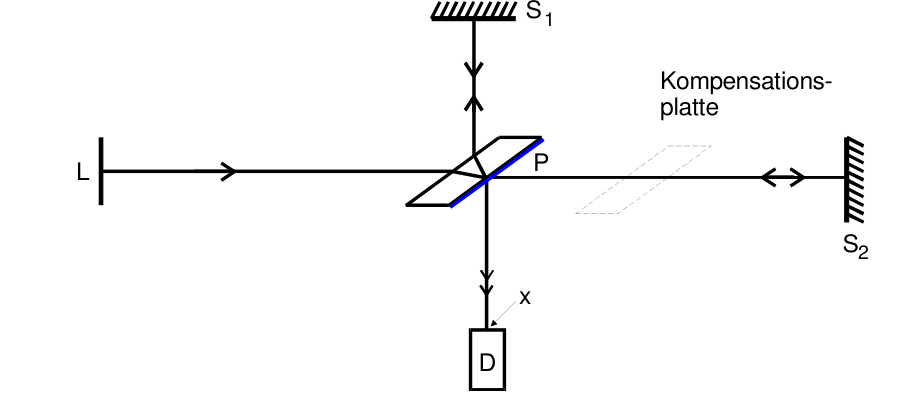
\includegraphics[width=0.9\textwidth]{18_v401/Abbildungen/Screenshot (4).png}
    \caption{Prinzipieller Aufbau des Michelson Interferometers \cite{man:v401}}
    \label{fig:schema_a}
\end{figure}
Ein Interferometer, teilt Licht in zwei Strahlen auf und führt sie wieder zusammen.
Durch die Veränderung eines der beiden Wege entsteht eine Veränderung des Interferenzmusters.
Aus dieser Veränderung können schließlich Rückschlüsse auf die Beschaffenheit der Lichtquelle gezogen werden.
Das Michelson Interferometer verwendet hierzu einen halbdurchlässigen Spiegel, der in einem \qty{45}{\degree}-Winkel 
zu dem Einfallendem Licht aufgestellt ist. 
Wie in Abbildung \ref{fig:schema_a} zu sehen wird der Lichtstrahl in zwei Arme aufgeteilt und von zwei Spiegeln wieder zurück reflektiert.
Der Strahl, der in $S_2$ reflektiert wird würde die Glasscheibe des Spiegels nur einmal durchlaufen im Gegensatz zu dem $S_1$ Strahl
der sie dreimal durchläuft.
Um einer Phasenverschiebung durch diesen Unterschied entgegenzuwirken wird eine Glasscheibe im gleichen Winkel 
auch in den Weg des $S_2$ Strahls gelegt.
Das Licht kann so am Detektor kohärent sein, wenn der Unterschied in den Weglängen der Arme kleiner der Kohärenzlänge ist.
Aus der Addition von zwei Wellen, bei der der eine Arm um d länger ist als der andere ergibt sich für die Intensität folgender Therm
\begin{align}
    I(d) = 2 \text{const} E_0^2 \left(1+ \cos\left(\frac{2\pi}{\lambda} 2d + \pi\right)\right).
\end{align}
Bei kontinuierlicher Vergrößerung um d schwankt I(d) also zwischen 0 und dem Maximalwert.
Verschiebt man den einen Spiegel in Strahlrichtung um das Stück $\Delta d$ und zählt die Anzahl der Helligkeitsmaxima $z$ ab
dann gilt folgender Zusammenhang:
\begin{align}
    \Delta d = z \frac{\lambda}{2}
    \label{eq:d_mod}
\end{align} 
Die Beschaffenheit des einen Armes kann auch durch einführung eines Materials mit unterschiedlichem Brechungsindex 
geschehen.
\begin{figure}
    \centering
    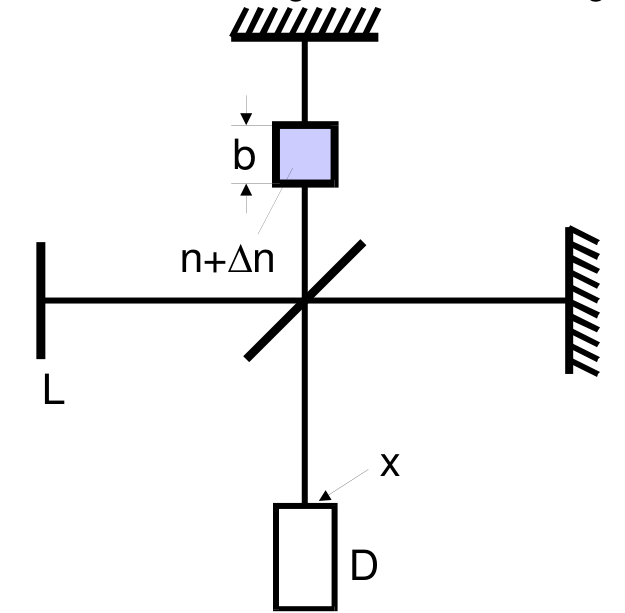
\includegraphics[width=0.4\textwidth]{18_v401/Abbildungen/Screenshot 2023-06-17 170025.png}
    \caption{Michelson-Interferometer zur Bestimmung eines Brechungsindex \cite{man:v401}}
    \label{fig:schema_b}
\end{figure}
Zum Beispiel kann die Luft aus einer Kammer (vgl. Abbildung \ref{fig:schema_b}) der tiefe $b$ herausgezogen werden,
wobei sich der Brechungsindexum $\Delta n$ verändert.
Mit $n$ als Brechungsindex der Luft und $n + \Delta n$ ergibt sich wiederum ein Gleichung für die Anzahl der Maximumsdurchläufe.
\begin{align}
    b \cdot \Delta n = \frac{z \lambda}{2}
    \label{eq:n_mod}
\end{align}
Aus der Thermodynamik und der idealen Gastheorie kann eine Gleichung für den Brechungsindex hergeleitet werden
\begin{align}
    n(p_0, T_0) = 1 + \Delta n(p, p') \frac{T}{T_0} \frac{p_0}{p-p'}.
    \label{eq:p_primed}
\end{align}
Hierbei sind $p_0$ und $T_0$ der Außendruck während der Druck in der Kammer von $p$ nach $p'$ geändert wird 
um die Änderung $\Delta n$ zu erreichen.

% Abhängigkeit von \alpha könnte hier noch rein... ist aber nicht so relevant verändert nach meinem 
% Verständnis nicht die Anzahl der Durchläufe. Außer vielleicht bei Störungen.
\input{Inhalte/B_Durchführung.tex}
\section{Auswertung}

\subsection{Gaußsche Fehlerfortpflanzung}

Wenn zu Messdaten die Standardabweichung bekannt ist, und mit diesen Messdaten weiter gerechnet werden soll,
wird die Gaußsche Fehlerfortpflanzung verwendet. 
Angenommen, es gibt $k$ Messwerte $x_i [i \in \mathbb{N}, i \leq k]$ mit den Standardabweichungen $\Delta x_i$
und eine abgeleitete Größe $f(x_i)$.
Dann ist der Fehler von $f$
\begin{align}
    \Delta f(x_i) = \sqrt{
    \left(\frac{\partial f}{\partial x_1} \Delta x_1\right)^2%
     + \left(\frac{\partial f}{\partial x_2} \Delta x_2\right)^2%
     + \dots%
     + \left(\frac{\partial f}{\partial x_k} \Delta x_k\right)^2%
    }.
    \label{eq:gauspflanz}
\end{align} 
Im Ergebnis ergibt sich der Mittelwert von $f$ mit der errechneten Abweichung $\overline{f} \pm \Delta f $.
Um Rechenfehler zu vermeiden, wird das Python \cite[]{python} Paket \texttt{uncertainties} \cite[][]{uncertainties} verwendet.
Hier wird die Fehlerfortpflanzung automatisch verrechnet, wenn die Variablen als \texttt{ufloat} definiert werden.

\subsection{Reichweite der Alpha-Strahlung}
In den beiden Messreihen errechnet sich die effektive Länge $x$ gemäß Gleichung \ref{eq:effektive_laenge}.
Da für den Druck jeweils ein Ablesefehler von \qty[]{5}{\milli\bar} angenommen wird, ergibt sich somit ein Fehler von 
\qty[]{3}{\mm} auf die Länge.
Für die Zählrate gibt es jeweils den Fehler $\Delta N = \sqrt{N}$.
Um von der Position \enquote{Channel} des Energiemaximums auf die entsprechende Energie zu kommen, wird der Dreisatz angewandt.
Dabei entspricht die Energie bei \qty{0}{\milli\bar} etwa \qty[]{4}{\mega\electronvolt}. 


\subsubsection[]{Erste Messreihe: 6 cm}
Die gemessenen und resultierenden Messgrößen bei einem Abstand von \qty[]{6}{\cm} sind in Tabelle \ref{tab:6cm} zu sehen.
Da die am Messgerät eingestellte Schwelle zwischen den Channels 696 und 697 liegt, werden die entsprechenden Werte
in der Auswertung nicht weiter berücksichtigt, um keine Ergebnisse zu verfälschen.
In der Tabelle sind die vernachlässigten Werte eingeklammert.

\begin{table}[H]
    \centering
    \caption{Druck $p$, effektive Länge $x$, Channel $C$, Energie $E$ sowie Zählrate $N$ bei einem Abstand von \qty[]{6}{\cm}.}
    \label{tab:6cm}
    \begin{tabular}{
        S[table-format=3.0] %druck
        S[table-format = 1.2] % x = eff laenge
        S[table-format=3.0] @{${}\pm{}$} S[table-format = 2.0] %N +- Fehler
        S[table-format=3.0] %channel
        S[table-format=1.2] % energie
    }
    \toprule
    {$p / \unit[]{\milli\bar}$} & {$x / \unit[]{\cm}$}
    & \multicolumn{2}{c}{$N / (1/\unit[]{\second})$} 
    & {$C$} & {$E / \unit[]{\mega\electronvolt}$} \\
    \midrule
     0  & 0.00 & 164 & 13 & 768 & 4.00 \\ 
     50 & 0.30 & 151 & 12 & 830 & 4.32 \\
    100 & 0.59 & 153 & 12 & 824 & 4.29 \\
    150 & 0.89 & 159 & 13 & 783 & 4.08 \\ 
    200 & 1.18 & 136 & 12 & 775 & 4.04 \\
    260 & 1.54 & 132 & 11 & 754 & 3.93 \\
    300 & 1.78 & 128 & 11 & 719 & 3.74 \\
    350 & 2.07 &  81 &  9 & 699 & 3.64 \\
    400 & 2.37 &  30 &  5 & {$(697)$} & {$(\num{3.63})$} \\
    450 & 2.67 &  14 &  4 & {$(697)$} & {$(\num{3.63})$} \\ 
    500 & 2.96 &   7 &  3 & {$(696)$} & {$(\num{3.62})$} \\
    560 & 3.32 &   6 &  2 & {$(696)$} & {$(\num{3.62})$} \\ 
    600 & 3.55 &   1 &  1 & {$(696)$} & {$(\num{3.62})$} \\
    650 & 3.85 &   2 &  2 & {$(696)$} & {$(\num{3.62})$} \\
    \bottomrule     
    \end{tabular}
\end{table}

\noindent
Wird $N$ gegen $x$ geplottet, ergibt sich Abbildung \ref{fig:rate_6cm}.
Mit Hilfe der Funktion \texttt{ODR} aus dem Python Paket \texttt{scipy} \cite[]{scipy}, 
die auf der Methode der kleinsten Quadrate beruht, 
wird eine Ausgleichsrechnung gemäß
\begin{align}
    N = a \cdot x + b
    \label{eq:lin}
\end{align}
durchgeführt.
Es ergeben sich die Parameter $a = \qty{-42.15 +- 6.69}{\per\cm\per\second}$ und $b = \qty{150.59 +- 22.35}{\per\second}$.
Hieraus lässt sich die mittlere Reichweite
\begin{align}
    R_\text{m} = \frac{N_\text{max} / 2 - b}{a} = \qty{1.63 +- 0.15}{\cm}
\end{align}
mit der maximalen Zählrate aus Tabelle \ref{tab:6cm} ermitteln.
Dies entspricht gemäß Gleichung \ref*{eq:reichweite} der Energie $E_\alpha = \qty{3.02 +- 0.19}{\mega\electronvolt}$.
% mittlere_reichweite =  1.63+/-0.15 cm
% zugehörige Energie =  3.02+/-0.19 MeV


\begin{figure}[H]
    \centering
    \includegraphics[height = 8.5cm]{build/reichweite_6cm_rate.pdf}
    \caption[]{Die Zählrate $N$ als Funktion der effektiven Länge $x$ beim Abstand von \qty{6}{\cm}.}
    \label{fig:rate_6cm}
\end{figure}

\noindent
Wird die Energie $E$ gegen die effektive Länge $x$ geplottet, ergibt sich Abbildung \ref{fig:energie_6cm}.
Hier ergibt eine lineare Ausgleichsrechnung analog zu \eqref{eq:lin} die Parameter $a = \qty{-0.260 +- 0.080}{\mega\electronvolt\per\cm}$
und $b = \qty{4.28 +- 0.10}{\mega\electronvolt}$.
Der Energieverlust beträgt also 
\begin{align}
    - \frac{dE}{dx} = -a = \qty{260 +- 80}{\kilo\electronvolt\per\cm}.
\end{align}

% a = -0.260 +- 0.080
% b = 4.277 +- 0.100
% energieverlust = (0.00260 +- 0.00080) MeV/m
% energieverlust = (260.29 +- 79.79) keV/cm

\begin{figure}[H]
    \centering
    \includegraphics[height = 8.5cm]{build/reichweite_6cm_energymax.pdf}
    \caption[]{Die Energie $E$ als Funktion der effektiven Länge $x$ beim Abstand von \qty{6}{\cm}.}
    \label{fig:energie_6cm}
\end{figure}



\subsection[]{Zweite Messreihe: 7 cm}
Die Auswertung verläuft komplett analog zur ersten Messreihe.
Die Zählrate geht bei diesem Abstand schneller gegen Null, sodass es hier keine Konflikte mit der am Messgerät eingestellten Schwelle gibt.
Es können also alle Werte in der Auswertung verwendet werden.
Die Messgrößen sind in Tabelle \ref{tab:7cm} zu sehen.

\begin{table}[H]
    \centering
    \caption{Druck $p$, effektive Länge $x$, Channel $C$, Energie $E$ sowie Zählrate $N$ bei einem Abstand von \qty[]{7}{\cm}.}
    \label{tab:7cm}
    \begin{tabular}{
        S[table-format=3.0] %druck
        S[table-format = 1.2] % x = eff laenge
        S[table-format=3.0] @{${}\pm{}$} S[table-format = 2.0] %N +- Fehler
        S[table-format=3.0] %channel
        S[table-format=1.2] % energie
    }
    \toprule
    {$p / \unit[]{\milli\bar}$} & {$x / \unit[]{\cm}$}
    & \multicolumn{2}{c}{$N / (1/\unit[]{\second})$} 
    & {$C$} & {$E / \unit[]{\mega\electronvolt}$} \\
    \midrule
     0  & 0.00 & 110 & 10 & 928 & 4.00 \\ 
     50 & 0.30 & 106 & 10 & 879 & 3.79 \\ 
    100 & 0.59 & 103 & 10 & 855 & 3.69 \\ 
    150 & 0.89 &  97 & 10 & 824 & 3.55 \\ 
    200 & 1.18 &  84 &  9 & 768 & 3.31 \\ 
    250 & 1.48 &  65 &  8 & 715 & 3.08 \\ 
    300 & 1.78 &  33 &  6 & 719 & 3.10 \\ 
    350 & 2.07 &   4 &  2 & 713 & 3.07 \\ 
    \bottomrule     
    \end{tabular}
\end{table}

\noindent
In Abbildung \ref{fig:rate_7cm} ist eine graphische Darstellung zwischen $x$ und $N$ zu sehen.
In diesem Fall ergeben sich die Parameter $a = \qty{-62.23 +- 6.85}{\per\cm\per\second}$ und $b= \qty{136.86 +- 12.44}{\per\second}$.
Daraus resultieren die Werte $R_\text{m} = \qty{1.32+-0.08}{\cm}$ und $E_α = \qty{2.62+-0.11}{\mega\electronvolt}$.

\begin{figure}[H]
    \centering
    \includegraphics[height = 8.5cm]{build/reichweite_7cm_rate.pdf}
    \caption[]{Die Zählrate $N$ als Funktion der effektiven Länge $x$ beim Abstand von \qty{7}{\cm}.}
    \label{fig:rate_7cm}
\end{figure}

\noindent
Der $x$-$E$-Plot ist in Abbildung \ref{fig:energie_7cm} zu sehen. 
Hier ergeben sich die Parameter $a = \qty{-0.482 +- 0.046}{\mega\electronvolt\per\cm}$ und $b= \qty{3.948 +- 0.058}{\mega\electronvolt}$.
Daraus folgt der Energieverlust $- {dE}/{dx} = \qty{482 +- 46}{\kilo\electronvolt\per\cm}$.


\begin{figure}[H]
    \centering
    \includegraphics[height = 8.5cm]{build/reichweite_7cm_energymax.pdf}
    \caption[]{Die Energie $E$ als Funktion der effektiven Länge $x$ beim Abstand von \qty{7}{\cm}.}
    \label{fig:energie_7cm}
\end{figure}





\subsection[]{Statistik des Zerfalls}
In Tabelle \ref{tab:stat} sind die gemessenen Zerfälle je 10 Sekunden bei einem Druck von \qty{0}{\milli\bar} zu sehen.

\begin{table}[H]
    \centering
    \caption{Intervallnummer $k$ und Anzahl der Zerfälle $N$ bei \qty{0}{\milli\bar}.}
    \label{tab:stat}
    \sisetup{table-format=2.0}
    \begin{tabular}{
        S %i von  1- 25
        S[table-format=4.0] %N von  1- 25
        S %i von 26- 50
        S[table-format=4.0] %N von 26- 50        
        S %i von 51- 75
        S[table-format=4.0] %N von 51- 75
        S[table-format=3.0] %i von 76-100
        S[table-format=4.0] %N von 76-100
    }
    \toprule
    {$k$} & {$N [1/(10\unit[]{\second})]$}
    & {$k$} & {$N [1/(10\unit[]{\second})]$}
    & {$k$} & {$N [1/(10\unit[]{\second})]$}
    & {$k$} & {$N [1/(10\unit[]{\second})]$} \\
    \cmidrule(lr){1-2}\cmidrule(lr){3-4}\cmidrule(lr){5-6}\cmidrule(lr){7-8}
     1 &  905 & 26 & 1022 & 51 &  941 &  76 & 1070 \\
     2 & 1017 & 27 & 1009 & 52 & 1027 &  77 &  929 \\
     3 &  983 & 28 & 1037 & 53 & 1014 &  78 &  950 \\
     4 & 1075 & 29 & 1035 & 54 &  980 &  79 &  913 \\
     5 &  955 & 30 &  974 & 55 & 1040 &  80 &  997 \\
     6 & 1004 & 31 & 1005 & 56 &  987 &  81 & 1044 \\
     7 &  916 & 32 &  985 & 57 &  995 &  82 &  965 \\
     8 &  952 & 33 & 1010 & 58 & 1082 &  83 & 1029 \\
     9 & 1021 & 34 &  936 & 59 &  957 &  84 &  981 \\
    10 & 1008 & 35 &  949 & 60 & 1066 &  85 &  956 \\
    11 &  989 & 36 &  964 & 61 & 1024 &  86 &  956 \\
    12 &  933 & 37 &  947 & 62 & 1002 &  87 &  964 \\
    13 & 1065 & 38 & 1057 & 63 & 1095 &  88 & 1023 \\
    14 & 1015 & 39 & 1069 & 64 & 1029 &  89 &  995 \\
    15 & 1038 & 40 & 1015 & 65 & 1032 &  90 & 1073 \\
    16 & 1043 & 41 & 1001 & 66 & 1007 &  91 & 1009 \\
    17 &  973 & 42 &  962 & 67 &  968 &  92 &  959 \\
    18 &  931 & 43 &  912 & 68 &  920 &  93 & 1008 \\
    19 & 1029 & 44 &  960 & 69 & 1011 &  94 & 1017 \\
    20 &  985 & 45 & 1002 & 70 & 1036 &  95 & 1025 \\
    21 & 1016 & 46 &  927 & 71 &  972 &  96 &  979 \\
    22 & 1020 & 47 &  973 & 72 &  977 &  97 &  949 \\
    23 & 1004 & 48 &  954 & 73 & 1037 &  98 & 1013 \\
    24 &  967 & 49 & 1028 & 74 &  951 &  99 &  956 \\
    25 &  977 & 50 & 1065 & 75 &  960 & 100 &  993 \\
    \bottomrule     
    \end{tabular}
\end{table}

\noindent
Es ergeben sich der Mittelwert $\overline{N} = 995 /(10\unit[]{\second})$ mit der Standardabweichung $\Delta N = 43/(10\unit[]{\second})$.
Anhand dieser Werte wird ein Histogramm erstellt, in dem zusätzlich eine Gauß- und eine Poisson-Verteilung zu sehen sind.
Das Histogramm ist in Abbildung \ref{fig:stat} zu sehen.
% ohne wurzel: 994.82 +- 42.75380217009945
% Mittelwert & Standardabw: 994.82 +- 3.15
% gerundete Werte: 995 +- 3
% Breite: 2.338973259083296

\begin{figure}[H]
    \centering
    \includegraphics[height = 8.5cm]{build/statistik.pdf}
    \caption[]{Histogramm der Messwerte mit einer Gauß- und einer Poissonverteilung.}
    \label{fig:stat}
\end{figure}
 
\section{Diskussion}
% Das Groundlevel schwankt


%Innenwiderstand Spannungsquelle

\printbibliography
\newpage

\section*{Anhang}
\addcontentsline{toc}{section}{\protect\numberline{}Anhang}

\begin{minipage}[t]{0.4\textwidth}
    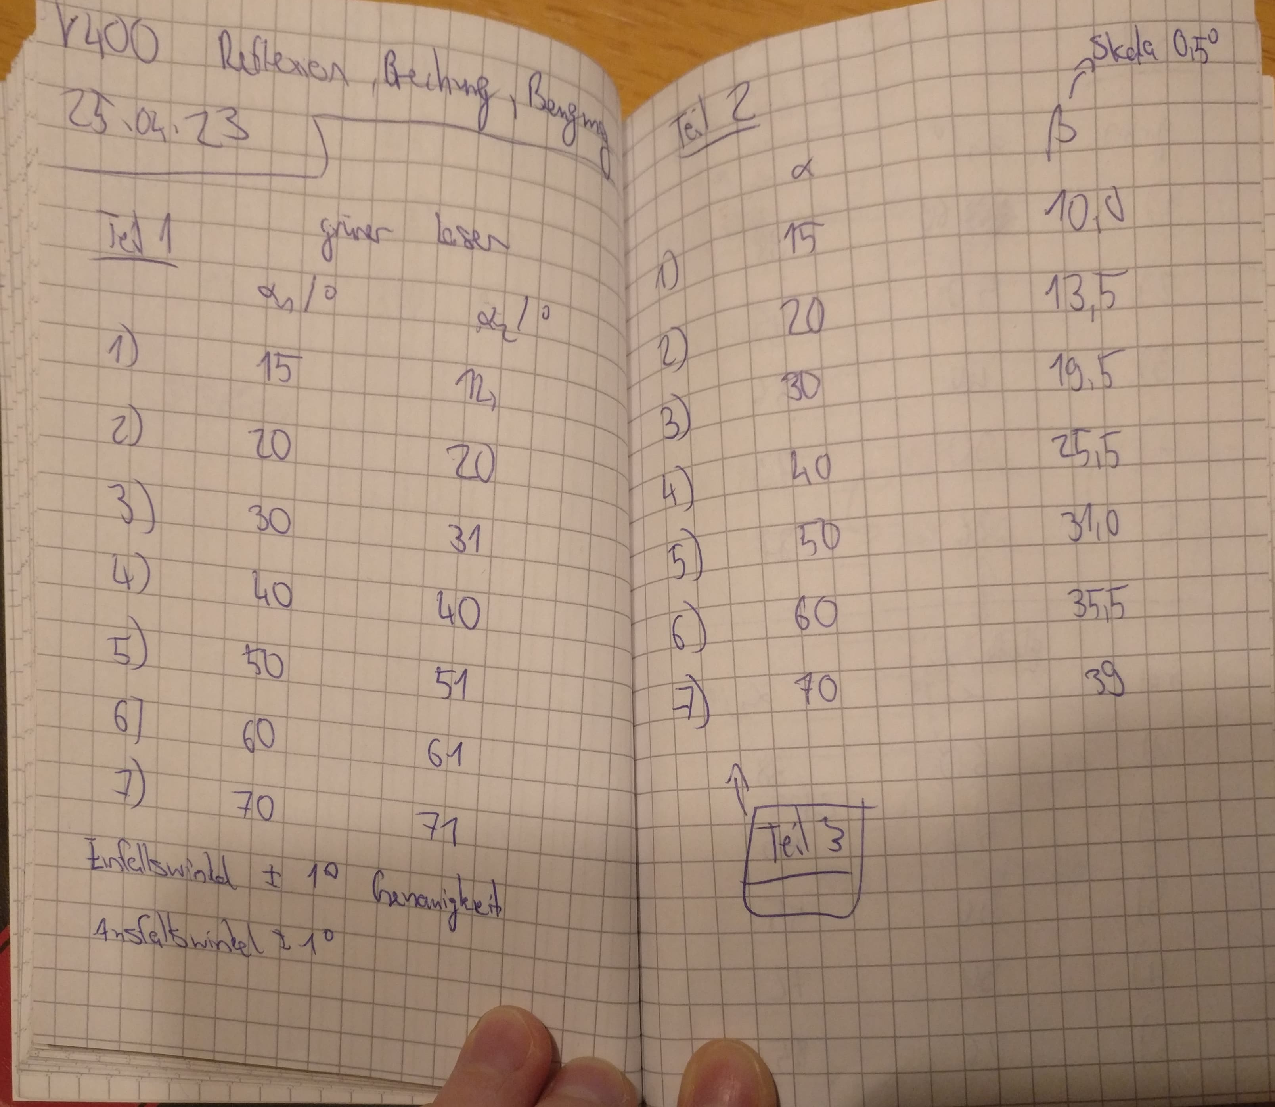
\includegraphics[height=4.5cm, page=1]{Abbildungen/v400_messdaten.pdf}
\end{minipage}
\begin{minipage}[t]{0.4\textwidth}
    \includegraphics[height=4.5cm, keepaspectratio, page=2]{Abbildungen/v400_messdaten.pdf}
\end{minipage}
\begin{minipage}[t]{0.4\textwidth}
    \includegraphics[height=4.5cm, page=3]{Abbildungen/v400_messdaten.pdf}
\end{minipage}
\begin{minipage}[t]{0.4\textwidth}
    \includegraphics[height=4.5cm, keepaspectratio, page=4]{Abbildungen/v400_messdaten.pdf}
\end{minipage}

\end{document}